\externaldocument{lit_review}
\externaldocument{facial_modelling_background}
\externaldocument{appendix}

\chapter{Blendshape Classification}\label{chap:classification}

This chapter shall discuss the problem of word level classification from blendshape parameters obtained from a dataset created with the VOCA model \cite{Cudeiro2019} processing audio from the LRW dataset \cite{Chung2016}.
Classification is performed with a Convolutional Neural Network architecture on 500 labels.
The model architecture, how performance is assessed and how the model has been tuned to maximise performance on a held out validation set is also discussed. 

\section{Problem Definition}
As with traditional lip reading problems, the end goal of VSR models using 3D temporal data is to correctly classify variable length input sequences at a sentence level.
However, before this problem can be tackled, the simpler problem of word level classification should be first approached to ensure that this is possible, before moving on to more advanced problems.
If word level classification cannot be achieved, it may be concluded that there is not a sufficient amount of information encoded in 3D temporal models for more complex problems to be solved with the current set of assumptions.

These assumptions include:
\begin{enumerate}
    \item Provided an appropriate dataset of 3D temporal facial scans of subjects speaking, a set of blendshape parameters which realistically represent the motions of speech can be found. \label{assumption:class_1}
    \item The blendshape parameters represent an encoding from which a classification model is able to make word level predictions. \label{assumption:class_2}
\end{enumerate}

\section{Generation of a 3D Lip Reading Dataset} \label{sec:dataset_gen}
In order to train any model, an appropriate dataset must exist upon which the model can be trained.
An appropriate dataset for word level prediction from blendshape parameters would consist of:
\begin{itemize}
   \item A large enough vocabulary that single instances of words with unique phonemes do not exist, as this would allow classification of these words to be too simple.
   \item Facial mesh recordings for all samples in the dataset, all of which brought into alignment to remove movement not related to speech.
   \item Principal blendshape axis which can be shown to contain useful interpolation for speech.
   \item The blendshape parameters corresponding to each sample for the given blendshape axis.
\end{itemize}

As discussed in section \ref{3D Datasets}, currently there exists no public datasets which have been created for the purpose of lip reading from 3D temporal data.
In addition to this, the datasets which have not been created with the purpose of lip reading but do contain 3D temporal data of speaking facial scans, are either not public in the case of Karras's model \cite{Karras2017a} or are unlabelled and too small to train a model effectively as is the case with the VOCASET \cite{Cudeiro2019}.
Both of these datasets also contain a large vocabulary, with too few samples of each word.
The VOCASET dataset could be labelled with the use of an automatic speech recognition model such as DeepSpeech as suggested in section \ref{3D Datasets}, however as the dataset was constructed to contain as much variation in speech sounds, so a degree of word repetition would offer little benefit, hence the lack of consistent word repetition.

In order to tackle the issue of an appropriate dataset not existing, two solutions exist.
The ideal solution would be to capture subjects speaking words from a set corpus using a 3D capture equipment, this solution was not a viable option for this project due to the specialised equipment required and the data processing required after data capture had been performed.
Another means of constructing the dataset would be to generate the data with an existing model which can convert an appropriate audio dataset to a series of facial meshes from which blendshape axis can be constructed and parameters recovered.
This can be achieved by processing audio from the LRW dataset \cite{Chung2016} though the VOCA model \cite{Cudeiro2019}.
The VOCA model claims to be able to generate realistic 3D facial motion from audio, as lip reading is notoriously difficult for humans, this is difficult to validate.
Assuming that the VOCA model does in fact generate realistic facial motion, the LRW dataset allows for a 3D dataset to be generated with a set corpus of the 500 words contained in the LRW dataset.

55,000 audio samples are taken from the LRW dataset with a uniform distribution of all labels, resulting in 110 samples for each label.
Audio samples from the LRW dataset are from ``in the wild'' scenarios \cite{Chung2016}, meaning that there is background noise and audio in the clip.
An sample of the word ``\textit{ABOUT}'' will contain the word ``\textit{ABOUT}'' within the audio sample, but will contain other speech either side of the clip.
Figure \ref{fig:LRW_About} shows such a sample labelled as ``\textit{ABOUT}'' in which the phrase ``talking about fair'' is spoken.

\begin{figure}[h]
    \centering
        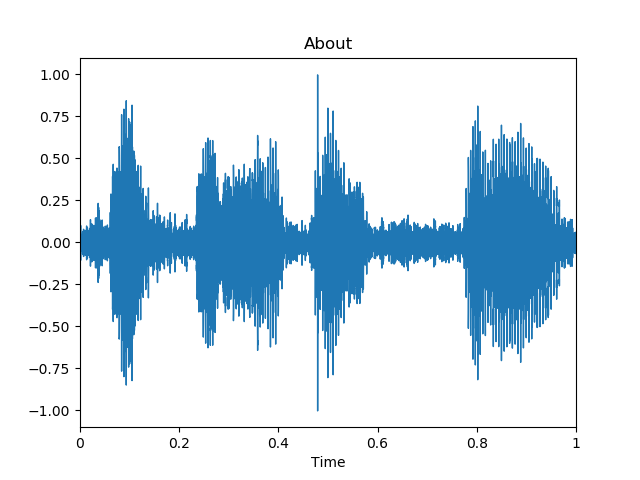
\includegraphics[width=0.7\textwidth]{figures/dataset/about.png}
    \caption{Audio Sample from LRW \cite{Chung2016} ``Talking About Fair''}\label{fig:LRW_About}
\end{figure}

The full LRW dataset contains 1000 training samples for each label, however due to the size of the VOCA model, processing 55000 samples (11\% of the full dataset) took roughly 8 days to process with the GPU acceleration of an Nvidia Tesla M60.
This is due to the size of the VOCA model, which incorporates the DeepSpeech model as a means of audio feature extraction.
In parallel to the generation of the 3D temporal data from the VOCA model, blendshape parameters were recovered as the facial scans were produced.
No significant decrease in the speed of data generation was observed running these tasks in parallel.

\subsection{Blendshape Axis Creation}
Ideally, all 55000 samples would be collected and the PCA would be performed on this to construct the blendshape axis.
However, due to disk space limitations a complete dataset of 55000 facial scans could not be collected at once due to the size of the generated facial meshes as this would total 2.365 million generated facial mesh data samples, each of which occupying around 185KB, requiring a total of 440GB of disc space.
To perform PCA on the generated facial meshes for blendshape axis (see section \ref{blendshapes}), the first 5000 facial mesh sequences were generated totalling 83 minutes of data and 215000 individual facial mesh data samples. 
Once PCA has been applied to a dataset of facial scans, the transformation matrix $\mat{W}$ is known.
$\mat{W}$ has columns of eigenvectors corresponding to eigenvalues, each of these eigenvectors represents the principal axis upon which can be interpolated.
These axes are the blendshapes axes and by interpolating along these axes by given amounts, motions of the facial mesh can be expressed in a low dimension.
The first blendshape axis corresponds to the largest eigenvalue, as that axis contains the largest amount of variation amongst the dataset.
The number of blendshapes which can be created will be limited by the number of positive non-zero eigenvalues found from PCA, however as each successive blendshape axis corresponds to a decreasingly small eigenvalue, the amount of variation in each successive axis decreases. 
This results in realistic reconstruction being able to be achieved with a relatively small number of blendshapes containing the majority of the variation within the dataset.
Examples of the First and Second Blendshape Axis from the first 5000 samples are shown in Figures \ref{fig:Blendshape_axis_1} and \ref{fig:Blendshape_axis_2} respectively, further examples can be viewed in the Appendix: Figure \ref{fig:Blendshape_axis_3}, \ref{fig:Blendshape_axis_4}.
These are constructed by interpolating along each axis individually by a fixed step amount.

\begin{figure}[h]
    \centering
    \begin{subfigure}[b]{0.24\textwidth}
        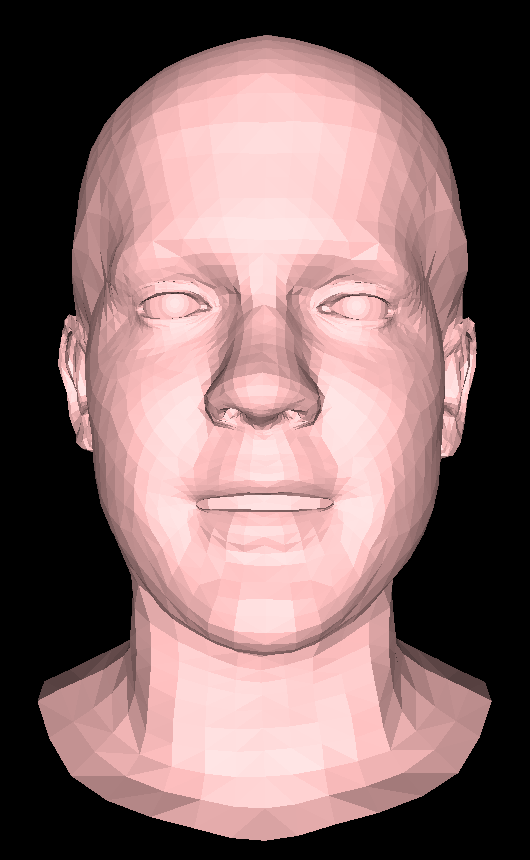
\includegraphics[width=\textwidth]{figures/blendshape_interp/1/00001.png}
    \end{subfigure}
    \begin{subfigure}[b]{0.24\textwidth}
        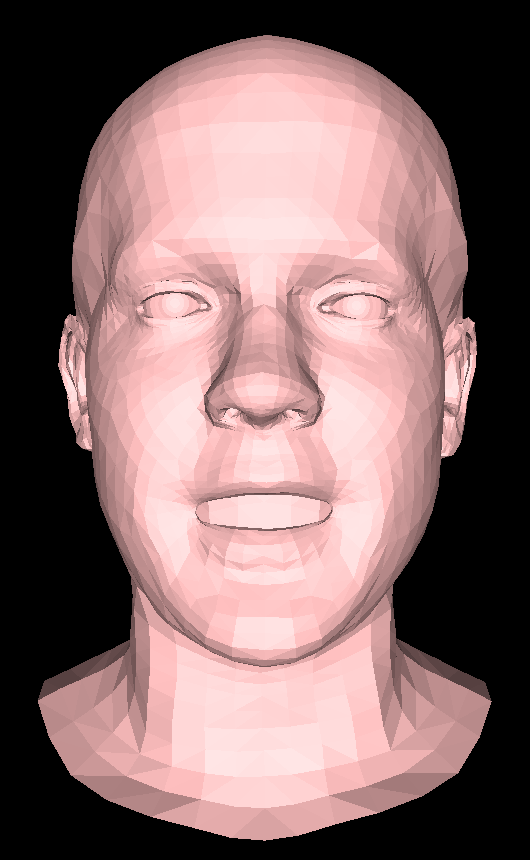
\includegraphics[width=\textwidth]{figures/blendshape_interp/1/00002.png}
    \end{subfigure}
    \begin{subfigure}[b]{0.24\textwidth}
        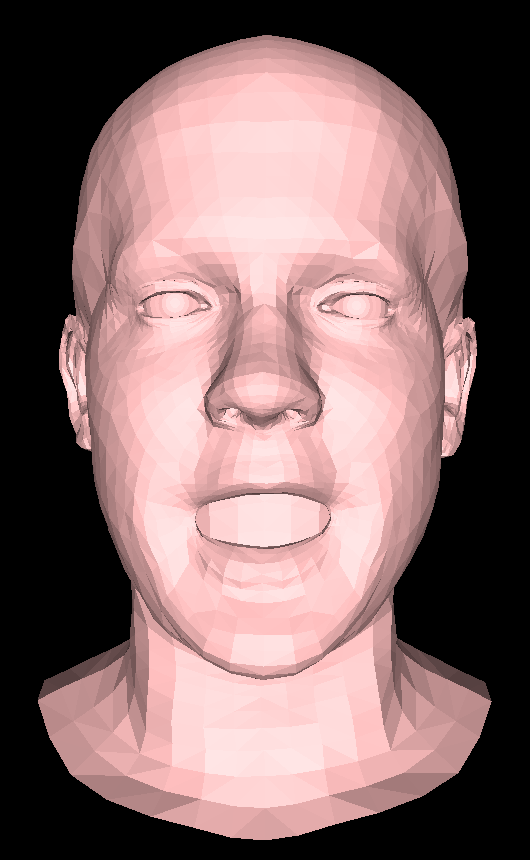
\includegraphics[width=\textwidth]{figures/blendshape_interp/1/00003.png}
    \end{subfigure}
    \begin{subfigure}[b]{0.24\textwidth}
        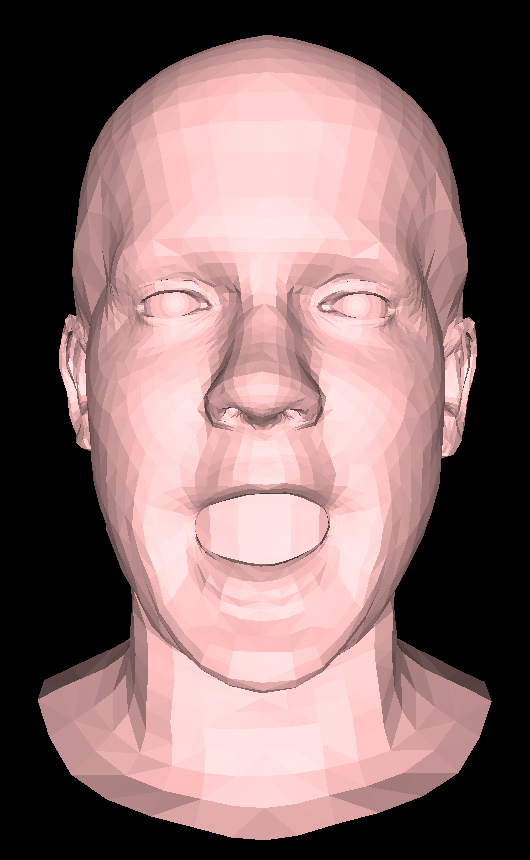
\includegraphics[width=\textwidth]{figures/blendshape_interp/1/00004.png}
    \end{subfigure}
    \caption{First Blendshape Axis Interpolation }\label{fig:Blendshape_axis_1}
\end{figure}
\begin{figure}[h]
    \centering
    \begin{subfigure}[b]{0.24\textwidth}
        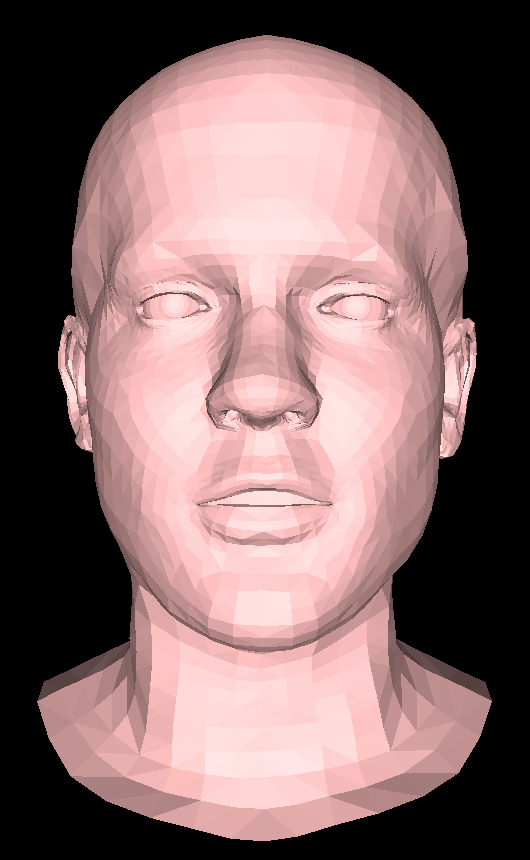
\includegraphics[width=\textwidth]{figures/blendshape_interp/2/00001.png}
    \end{subfigure}
    \begin{subfigure}[b]{0.24\textwidth}
        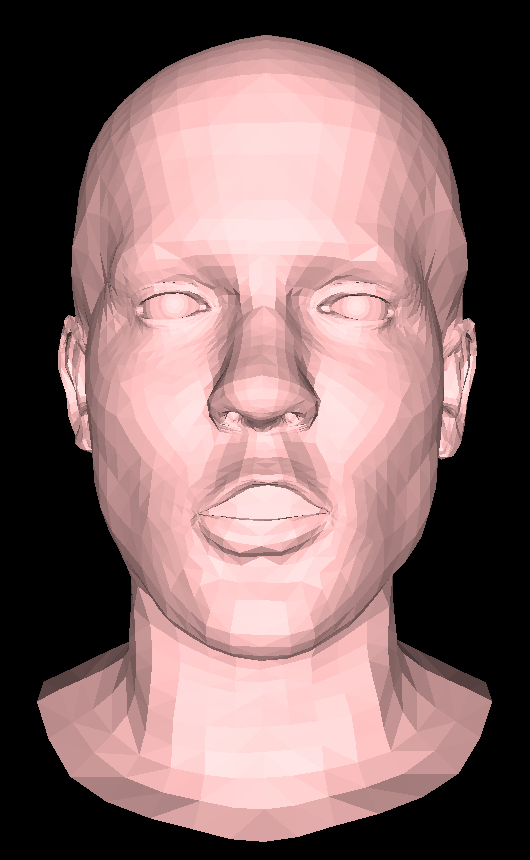
\includegraphics[width=\textwidth]{figures/blendshape_interp/2/00002.png}
    \end{subfigure}
    \begin{subfigure}[b]{0.24\textwidth}
        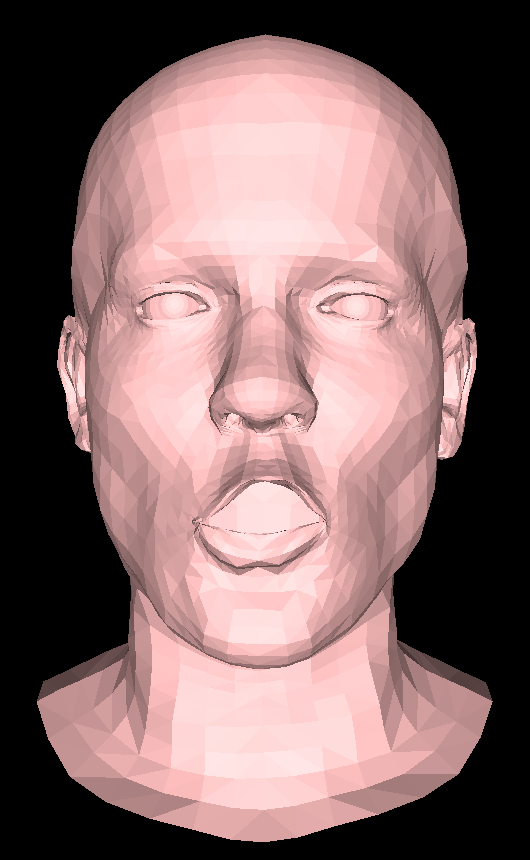
\includegraphics[width=\textwidth]{figures/blendshape_interp/2/00003.png}
    \end{subfigure}
    \begin{subfigure}[b]{0.24\textwidth}
        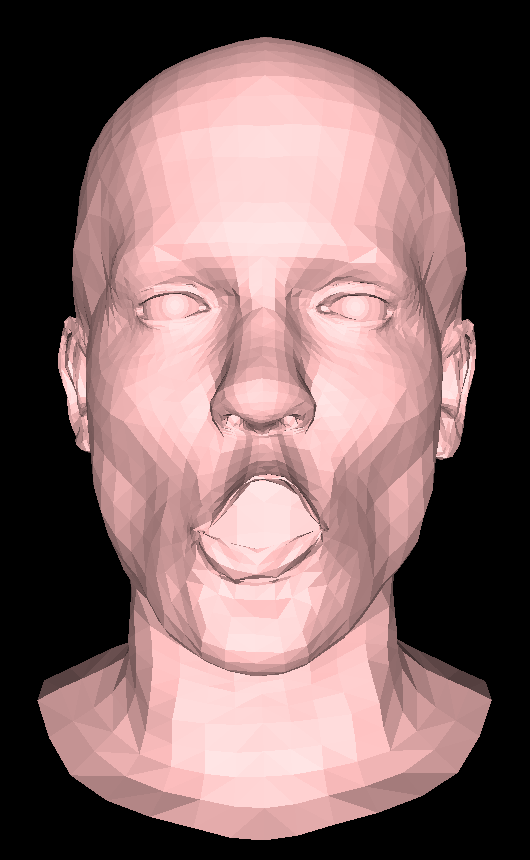
\includegraphics[width=\textwidth]{figures/blendshape_interp/2/00004.png}
    \end{subfigure}
    \caption{Second Blendshape Axis Interpolation}\label{fig:Blendshape_axis_2}
\end{figure}

\subsection{Blendshape Parameter Recovery} \label{sec:blendshape_recovery}
Given a template mesh $\mat{M} \in \mathbb{R}^{(N \times 1)}$ upon which to interpolate, where $N = 3n$ and $n$ represents the number of vertex points in the facial mesh, each of which have an $x, y$ and $z$ coordinate value and Blendshape Axis $\mat{W} \in \mathbb{R}^{(N \times d)}$ as described in section \ref{sec:pca}, where the $d$ first principal axis have been kept, representing the axis along which the template mesh $\mat{M}$ can be interpolated.

\begin{equation*}
    \mat{M} = \begin{bmatrix} 
                x_{1}, &
                y_{1}, &
                z_{1}, &
                \dots, &
                x_{n}, &
                y_{n}, &
                z_{n}
               \end{bmatrix}^\top,
    \quad
    \mat{M} \in \mathbb{R}^{N\times 1},
    \quad
    N = 3n,
\end{equation*}
\quad
\begin{equation*}
    \mat{W} = [
               \bm{w_1}, \dots, \bm{w_d}
              ],
    \quad
    \mat{W} \in \mathbb{R}^{(N \times d)}
\end{equation*}
\quad
\begin{equation*}
    \bm{w_i} = \begin{bmatrix} 
                x_{1}, &
                y_{1}, &
                z_{1}, &
                \dots, &
                x_{n}, &
                y_{n}, &
                z_{n}
    \end{bmatrix}^\top
\end{equation*}

Given subsequent frames $\mat{M}^{\prime}$ which deviate the facial mesh from $\mat{M}$, $\mat{M}^{\prime}$ can be expressed by equation \ref{eq:mesh_interp}, where $\bm{\Lambda}$ is a vector containing Blendshape parameters.

\begin{equation}\label{eq:mesh_interp}
    \mat{M}^{\prime} = \mat{M} + \mat{W} \mat{\Lambda}
\end{equation}
\quad
\begin{equation*}
    \mat{\Lambda} = \begin{bmatrix}
        \lambda_1, &
        \dots, &
        \lambda_d
    \end{bmatrix}^\top
\end{equation*}

The blendshape parameters $\lambda_i$ can be found by rearranging equation (\ref{eq:mesh_interp}) and solving for $\bm{\Lambda}$ as shown in equation (\ref{eq:mesh_interp_lambda}).
The solution to this can be found by finding the pseudo-inverse for the Blendshape Axes $\mat{W}$.

\begin{equation}\label{eq:mesh_interp_lambda}
    \mat{\Lambda} = \mat{W}^{-1}(\mat{M}^{\prime} - \mat{M})
\end{equation}

\subsection{Dataset Split}
The dataset consists of 55000 samples.
This is split into Training, Validation and Test data with 20000/20000/15000 data points respectively.
When training the model the Training data will be shown to the model, the model will then be evaluated on the Validation data which allows model hyperparameters to be adjusted to improve performance on this dataset.
To ensure that the model has not been optimised just for the Validation data and can generalise to unseen data, the final performance is reported on the Test data, which is never evaluated on until the model has been tuned to optimum performance on the Validation data.

\section{Data Preprocessing}
To aid training, the dataset is normalised to a range of [0,1] using equation (\ref{eq:normalise}) where $x_{min}$ and $x_{max}$ are the smallest and largest values in the dataset respectively (Figure \ref{fig:hist_norm}).
While each Blendshape Axis is separate from one another, normalisation should be performed on all parameters as a whole to preserve information on the variation found in each Blendshape Axis relative to one another.
As described by PCA in section \ref{sec:pca}, the variation in each subsequent principal axis decreases which can be seen in Figure \ref{fig:hist_norm}.

\begin{equation}\label{eq:normalise}
   x^\prime = \frac{x - x_{min}}{x_{max} - x_{min}} 
\end{equation}

\begin{figure}[h!]
    \centering
    \begin{subfigure}[b]{0.49\textwidth}
        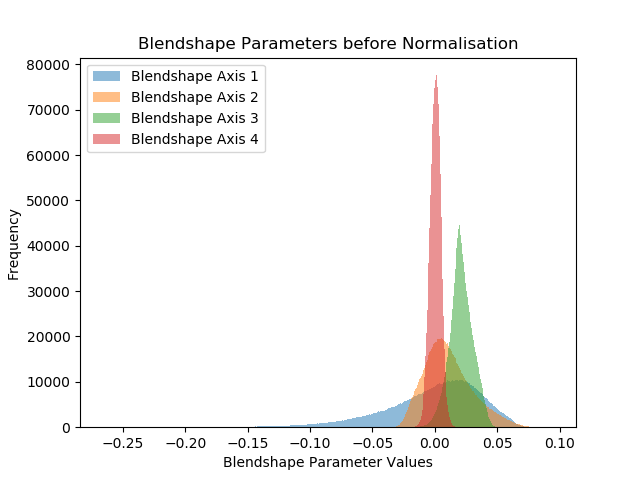
\includegraphics[width=\textwidth]{figures/dataset/shape_params_unnormalised_hist.png}
        \caption{Unnormalised}\label{fig:hist_unnorm}
    \end{subfigure}
    \begin{subfigure}[b]{0.49\textwidth}
        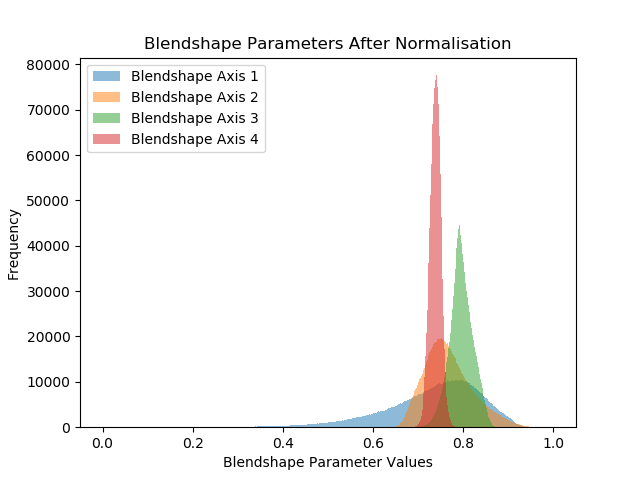
\includegraphics[width=\textwidth]{figures/dataset/shape_params_normalised_hist.png}
        \caption{Normalised}\label{fig:hist_norm}
    \end{subfigure}
    \caption{Blendshape Parameter Histograms}
\end{figure}

\section{Assessment of Model Performance}\label{sec:class_assessment}
In order to assess the performance of the models in the task of word level classification, several metrics exist which could be used.
The chosen metrics are the model accuracy and the Levenshtein Distance.
The accuracy gives a measure of how frequently the model correctly predicts the word while the Levenshtein Distance represents how far the incorrect predictions are from the correct words.

\subsection{Accuracy}
The accuracy of a model is the ratio between the number of predicted labels made by the model which are correct and the total number of predictions.
Accuracy is an appropriate metric in the instance when the dataset is balanced, that is to say that there are an equal number of all labels in the dataset.

If the dataset is unbalanced, the accuracy of a model is less informative.
For example, in the scenario where there is a dataset with two labels \textit{A} and \textit{B} with the data being unbalanced such that label \textit{A} occurs 9 times for frequently than label \textit{B}.
A model which achieves 90\% accuracy on this dataset may be correctly labelling all data 90\% of the time, or it may be labelling all data samples as label \textit{A} without learning anything about the dataset and achieving the same accuracy.

For unbalanced data the F1-Score metric is more useful as this will remain low when a single label class is frequently being incorrectly predicted.
However, as the dataset this problem is concerned with is balanced, this shall not be discussed.

\subsection{Levenshtein Distance}
The Levenshtein Distance is a character level distance between two words defined as the minimum number of single character edits required to make the two the same \cite{Levenshtein1966}.
Single character edits are described as removing a character, substituting for another character and adding a new character.
In the example shown in Figure \ref{fig:levenshtein}
This was used by Chung et al. in \cite{Cheng2016}, although it was defined as the character-level edit distance (section \ref{sec:lip_reading_models}).
This can be calculated for each model prediction and the average character-level edit distance can be found for the model as a whole, or per label.

\begin{figure}[h!]
\centering
    \begin{tabular}{c c c c c l }
        \multicolumn{1}{ c }{} & \\
        A & B & U & S & E & \\
        A & B & O & U & T & \\
        \cline{1-5}
        & & & & & \multicolumn{1}{l}{\textbf{Operation}} \\
        \cline{1-5}
        A & B & U & T & - & Remove O \\
        \cline{1-5}
        A & B & U & S & - & Substitute T for S\\
        \cline{1-5}
        A & B & U & S & E & Add E\\
        \cline{1-5}
    \end{tabular} 
    \caption{Levenshtein Distance Example}\label{fig:levenshtein}
\end{figure}

\section{Model Architecture}

\subsection{Multiple Towers Classification Model}
The first model is based on the Multiple Towers architecture used in \cite{Chung2016} used for lip reading on 2D temporal data with the LRW dataset described in Section \ref{sec:lip_reading_models}.
This is a CNN architecture which firstly applies a convolutional layer to the input image frames separately before concatenating the output feature maps and proceeding to convolve over the time domain.
The original Multiple Towers architecture can be seen in Figure \ref{fig:LRW_Multiple_Towers} while the architecture adapted from this design for prediction from blendshape parameters is shown in Figure \ref{fig:Blendshape_Multiple_Towers}

\subsubsection{Model Input} \label{sec:classification_inputs}
The model inputs are in the form of blendshape parameter values for each frame in the motion sequence.
These represent the interpolation from the template mesh as described in section \ref{sec:blendshape_recovery} for each time frame.
For a duration of one second there are 43 frames, 4 blendshape parameters per frame and a single channel dimension, such that the input to the model is $\mat{x} \in \mathbb{R}^{1 \times 4 \times 43}$

\subsubsection{Loss Function}
The model is trained with the Negative Log Likelihood (NLL) on 500 class labels for each of the labels in the dataset.
The model makes word level predictions with the LogSoftmax activation function applied to the final layer of the model.

\subsubsection{Model Architecture} \label{sec:classification_model_arch}
Similar to the architecture proposed by Chung et al. \cite{Chung2016}, the first convolutional layers do not convolve over the time domain by using 3x1 kernels which do not have a receptive field across the time domain.
These two layers reduce the input shape from $[1 \times 4 \times 43]$ to $[512 \times 1 \times 43]$, encoding the 4 blendshape parameters into a single value across multiple channels, allowing the single dimension to be collapsed and 1D convolutional layers to be used for subsequent layers.

The Multiple Towers architecture used by Chung et al. featured max pooling layers to reduce the size of feature maps.
As a linear layer is to be used at the final layer of the model to facilitate label prediction with a LogSoftmax activation function, it is desirable to reduce the size of the feature maps to prevent the linear layer having too many parameters as this becomes difficult to train and can lead to overfitting.
Max pooling layers reduce the size of feature maps in the network, only retaining the information which is of the most use to the model.

In order to aid in the training of the model, batch normalisation is applied after convolutional layers in all cases except for the final convolutional layer.
Similarly, dropout was applied to all but the final convolution layer in order to assist the model from overfitting the training data.
During training, the model suffered from significant overfitting to the training data, dropout was applied and assist in the prevention of this.
In addition to dropout, weight decay was also used to improve performance on the validation data.
Early stopping was used to prevent the model learning to overfit further on the training data.
This was achieved by keeping a running average of the loss on validation data of the previous 10 epochs, training was stopped once the validation loss stopped decreasing (see Figure \ref{fig:blendshape_multi_tower_loss}).

A detailed breakdown of the model specification can be seen in Table \ref{table:multi_towers_classifier}.
The hyperparameters which provided the optimum results on the validation data are shown in Table \ref{table:multi_towers_classifier_hyperparameters} 

\begin{figure}[h!]
    \centering
        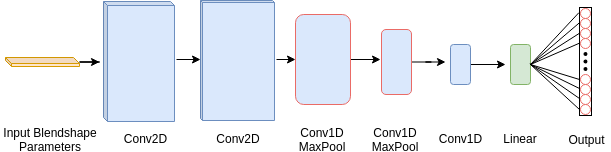
\includegraphics[width=0.9\textwidth]{figures/classification/blendshape_multi_tower_arch.png}
    \caption{Multiple Towers Classification Architecture}\label{fig:Blendshape_Multiple_Towers}
\end{figure}
\quad

\begin{table}[h!]
\centering
    \begin{tabular}{l | r | r | r | l | r | l}
    \textbf{Layer} & \textbf{Output} & \textbf{Kernel} & \textbf{Stride} & \textbf{Batch Norm} & \textbf{Dropout} & \textbf{Activation} \\ \hline
    Conv2D & 512x2x43 & 3x1 & 1x1 & True & 0.2 & ReLU \\ \hline
    Conv2D & 512x1x43 & 3x1 & 1x1 & True & 0.2 & ReLU \\ \hline
    Conv1D & 256x41 & 3 & 1 & True & 0.2 & ReLU \\ \hline
    MaxPool & 128x20 & 3 & 2 & - & - & - \\ \hline
    Conv1D & 64x18 & 3 & 1 & True & 0.2 & ReLU \\ \hline
    MaxPool & 64x9 & 3 & 2 & - & - & - \\ \hline
    Conv1D & 64x7 & 3 & 1 & False & 0.0 & ReLU \\ \hline
    Linear & 500 & - & - & False & 0.0 & LogSoftmax \\
    \end{tabular} 
    \caption{Multiple Towers Model Architecture}\label{table:multi_towers_classifier}
\end{table}
\quad

\begin{table}[h!]
\centering
    \begin{tabular}{l | r | r | r}
    \textbf{Optimisation} & \textbf{Learning Rate} & \textbf{Weight Decay} & \textbf{Batch Size} \\ \hline
    RMSprop & 0.0002 & 0.001 & 128 \\
    \end{tabular} 
    \caption{Multiple Towers Model Hyperparameters}\label{table:multi_towers_classifier_hyperparameters}
\end{table}


\subsection{Blendshape Channels Classification Model}
The second model applied to this task is not directly inspired by any existing model architecture.
Unlike the Multiple Towers Model, this model convolves over the time domain throughout the whole depth of the model and treats each blendshape axis as a separate channel to the input of the model, thus the model shall be referred to as the Blendshape Channels Model.
As with the previous classification model, NLL is used as a loss function.

\subsubsection{Model Input}
The model inputs, as before are in the form of blendshape parameters values corresponding to frames in the motion sequence.
Unlike the previous model, each blendshape axis is treated as a separate input channel, such that the input data is in the form $\mat{x} \in \mathbb{R}^{4 \times 43}$.
Treating the blendshape axes as separate channels allows the model to extract information from them separately while considering the time domain for each.

TODO, some of this may need to be moved to discussion section.

\subsubsection{Model Architecture}
The Blendshape Channel model is a CNN architecture convolving over the time domain of the input data throughout the whole depth of the model.
Reducing the length of the feature maps as the model deepens, while increasing the number of channels in the feature maps to allow for more fine details to be extracted from the data.

In order to reduce the length of the feature maps in the model, max pooling layers are applied after the 3\textsuperscript{rd} and 5\textsuperscript{th} convolutional layers.
As with the Multiple Towers Model, this forces the model to discard information which is of less importance, while reducing the size of the feature maps.

The final convolutional layer reduces the number of channels in the output feature map in order to reduce the number of parameters in the output linear layer for word level predictions with the LogSoftmax activation function.
Full model specification are shown in Table \ref{table:blendshape_channels_classifier}.
Similar to the Multiple Towers Model, batch normalisation is applied to aid in stabilising the training of the model, while dropout did not improved the performance on the validation data.
The model was tuned on the validation data to with the hyperparameters shown in Table \ref{table:blendshape_channels_classifier_hyperparameters}.

\begin{figure}[h!]
    \centering
        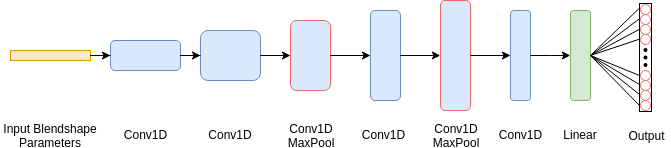
\includegraphics[width=0.9\textwidth]{figures/classification/blendshape_channel_arch.png}
    \caption{Blendshape Channels Classification Architecture}
\end{figure} \label{fig:Blendshape_Channel_Classifier}
\quad

\begin{table}[h!]
\centering
    \begin{tabular}{ l | r | r | r | l | r | l}
    \textbf{Layer} & \textbf{Output} & \textbf{Kernel} & \textbf{Stride} & \textbf{Batch Norm} & \textbf{Dropout} & \textbf{Activation} \\ \hline
    Conv1D & 4x43 & 3 & 1 & True & 0.0 & ReLU \\ \hline
    Conv1D & 32x41 & 3 & 1 & True & 0.0 & ReLU \\ \hline
    Conv1D & 64x39 & 3 & 1 & True & 0.0 & ReLU \\ \hline
    MaxPool & 128x18 & 3 & 2 & - & - & - \\ \hline
    Conv1D & 256x16 & 3 & 1 & True & 0.0 & ReLU \\ \hline
    Conv1D & 512x14 & 3 & 1 & True & 0.0 & ReLU \\ \hline
    MaxPool & 512x7 & 2 & 2 & - & - & - \\ \hline
    Conv1D & 256x5 & 3 & 1 & False & 0.0 & ReLU \\ \hline
    Linear & 500 & - & - & False & 0.0 & LogSoftmax \\
    \end{tabular} 
    \caption{Blendshape Channels Model Architecture}
\end{table}\label{table:blendshape_channels_classifier}
\quad

\begin{table}[h!]
\centering
    \begin{tabular}{l | r | r | r}
    \textbf{Optimisation} & \textbf{Learning Rate} & \textbf{Weight Decay} & \textbf{Batch Size} \\
    \hline
    RMSprop & 0.00005 & 0.005 & 128 \\
    \end{tabular} 
    \caption{Blendshape Channels Model Hyperparameters}
\end{table}\label{table:blendshape_channels_classifier_hyperparameters}

\section{Results}
Examining the training losses and validation losses for both models show that despite tuning on the Validation dataset, the model remains to overfit to the Training data considerably.
This can be seen from the continued reduction in training loss while the validation loss plateaus for both models (Figures \ref{fig:multiple_towers_training}, \ref{fig:channels_training}).

\begin{figure}[h!]
    \centering
    \begin{subfigure}[b]{0.49\textwidth}
        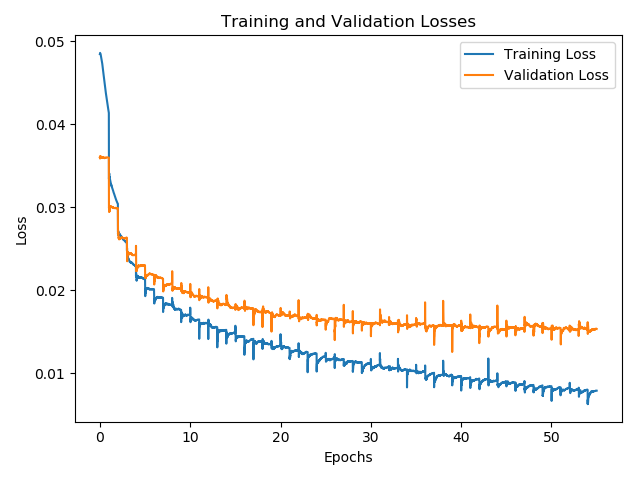
\includegraphics[width=\textwidth]{figures/classification/blendshape_multi_tower_loss.png}
        \caption{Losses}\label{fig:blendshape_multi_tower_loss}
    \end{subfigure}
    \begin{subfigure}[b]{0.49\textwidth}
        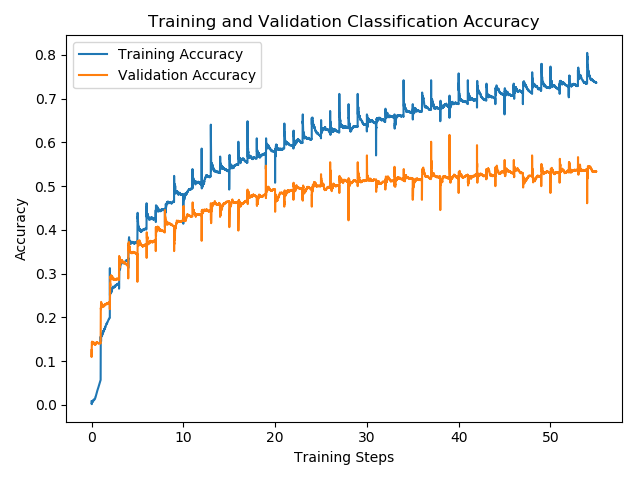
\includegraphics[width=\textwidth]{figures/classification/blendshape_multi_tower_acc.png}
        \caption{Accuracy}\label{fig:blendshape_multi_tower_acc}
    \end{subfigure}
    \caption{Multiple Towers Training}\label{fig:multiple_towers_training}
\end{figure}

\begin{figure}[h!]
    \centering
    \begin{subfigure}[b]{0.49\textwidth}
        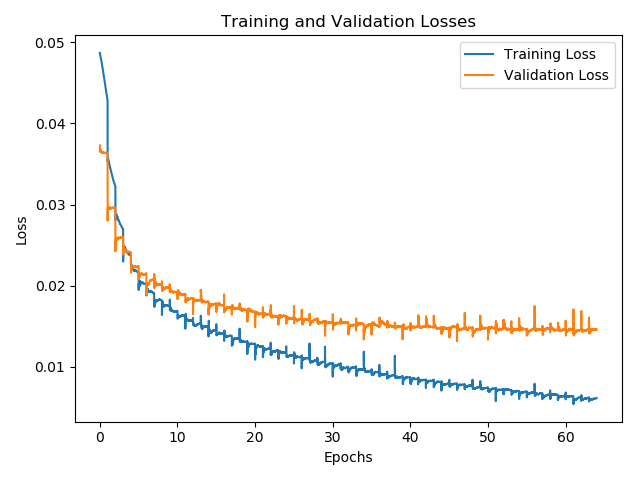
\includegraphics[width=\textwidth]{figures/classification/blendshape_channel_loss.png}
        \caption{Losses}\label{fig:blendshape_channel_loss}
    \end{subfigure}
    \begin{subfigure}[b]{0.49\textwidth}
        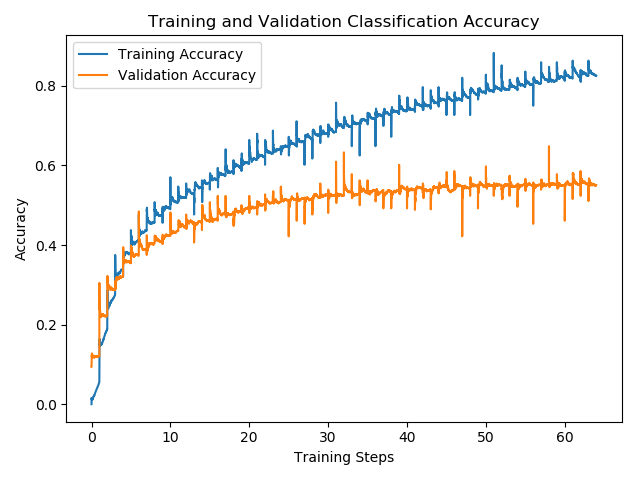
\includegraphics[width=\textwidth]{figures/classification/blendshape_channel_acc.png}
        \caption{Accuracy}\label{fig:blendshape_channel_acc}
    \end{subfigure}
    \caption{Blendshape Channels Training}\label{fig:channels_training}
\end{figure}

A direct comparison of the models on the Validation data shows that the Blendshape Channel architecture slightly outperforms the Multiple Towers architecture throughout training (Figure \ref{fig:classification_training}).
The final model accuracy values for each dataset split is shown in Table \ref{table:classification_test_accuracy}.
Evaluation on the Test data concludes that the Blendshape Channels model is consistent outperforms, while the margin between the two models remains small.

\begin{figure}[h!]
    \centering
    \begin{subfigure}[b]{0.49\textwidth}
        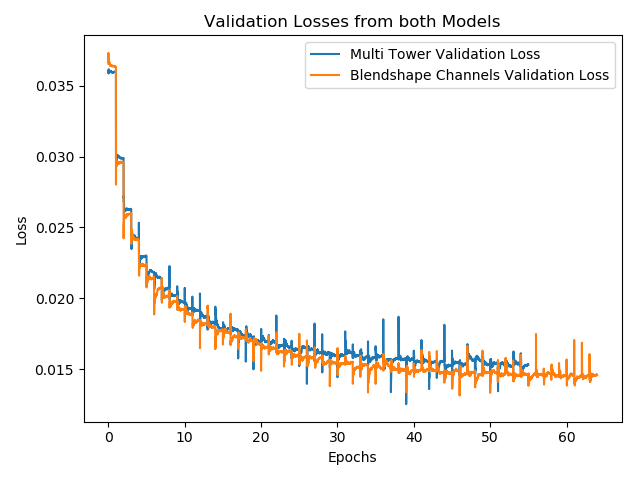
\includegraphics[width=\textwidth]{figures/classification/both_models_val_loss.png}
        \caption{Losses}\label{fig:both_models_val_loss}
    \end{subfigure}
    \begin{subfigure}[b]{0.49\textwidth}
        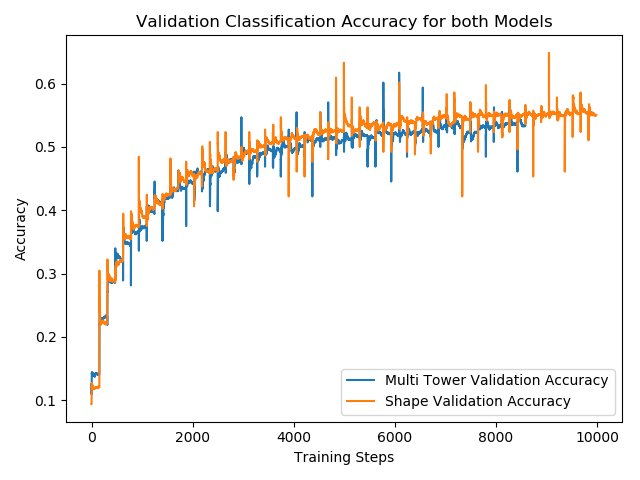
\includegraphics[width=\textwidth]{figures/classification/both_models_val_acc.png}
        \caption{Accuracy}\label{fig:both_models_val_acc}
    \end{subfigure}
    \caption{Model Training Comparison}\label{fig:classification_training}
\end{figure}

\begin{table}[h!]
\centering
    \begin{tabular}{l | l | l | l }
    & \textbf{Train} & \textbf{Validation} & \textbf{Test} \\ \hline
    \textbf{Multiple Towers} & 0.7911 & 0.5333 & 0.5276 \\
    \textbf{Blendshape Channels} & 0.8544 & 0.5504 & 0.5461 \\
    \end{tabular} 
    \caption{Blendshape Classification Models Test Data Accuracy}
\end{table}\label{table:classification_test_accuracy}

Examining word level classification accuracy on the Test dataset (Figure \ref{fig:both_models_word_acc}) shows that both models perform similarly across all labels.
A more detailed evaluation of the 1\textsuperscript{st} percentile of the Test dataset shown in Figure \ref{fig:both_models_percentile_word_acc} highlights that the label which was most poorly predicted was the same for both models (\textit{`GOING'}).
While the second worse predicted label in both cases achieved 9.09\% and 8.33\% for the Multiple Towers and Blendshape Channels models respectively, far higher than the 0.2\% accuracy which would be achieved by a model which makes a purely random guess from 500 labels.

\begin{figure}[h!]
    \centering
    \begin{subfigure}[b]{0.49\textwidth}
        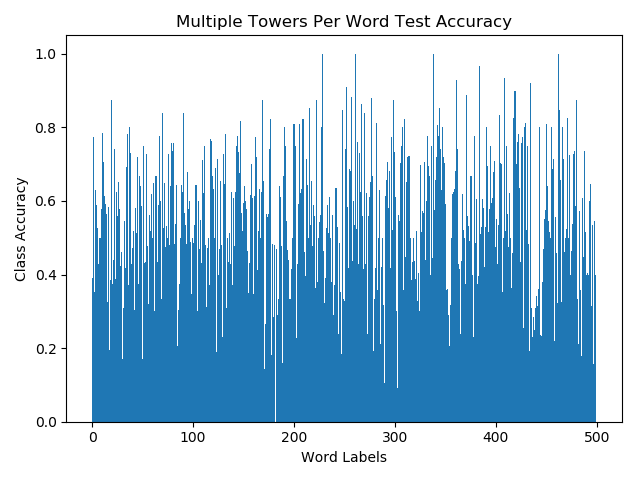
\includegraphics[width=\textwidth]{figures/classification/blendshape_multi_tower_class_acc.png}
        \caption{Multiple Towers}\label{fig:multiple_towers_word_acc}
    \end{subfigure}
    \begin{subfigure}[b]{0.49\textwidth}
        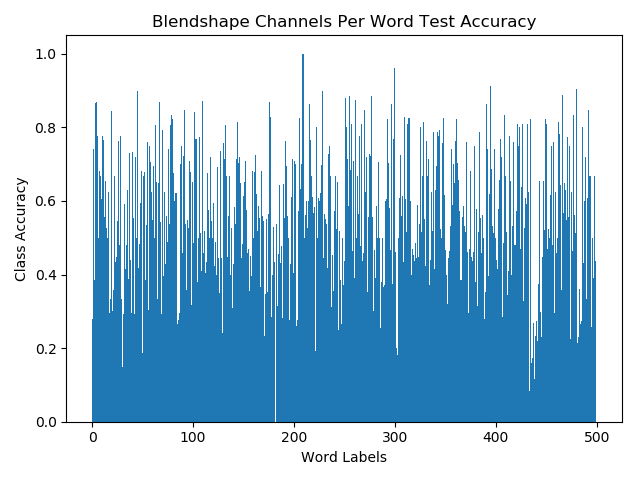
\includegraphics[width=\textwidth]{figures/classification/blendshape_channel_class_acc.png}
        \caption{Blendshape Channels}\label{fig:channels_word_acc}
    \end{subfigure}
    \caption{Per Word Test Accuracy}\label{fig:both_models_word_acc}
\end{figure}

\begin{figure}[h!]
    \centering
    \begin{subfigure}[b]{0.49\textwidth}
        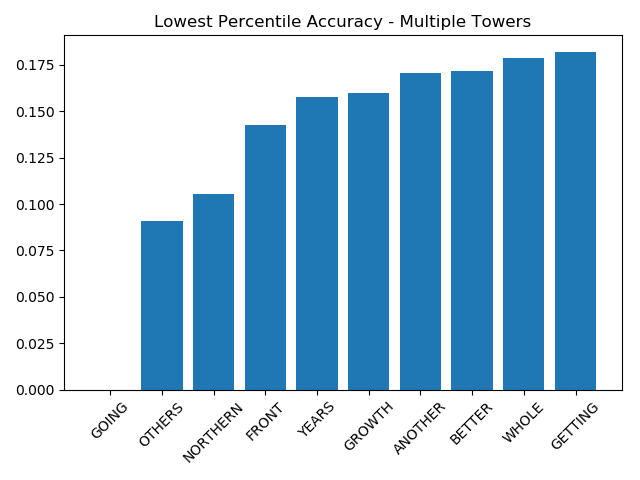
\includegraphics[width=\textwidth]{figures/classification/blendshape_multi_tower_percentile_class_acc.png}
        \caption{Multiple Towers}\label{fig:multiple_towers_percentile_word_acc}
    \end{subfigure}
    \begin{subfigure}[b]{0.49\textwidth}
        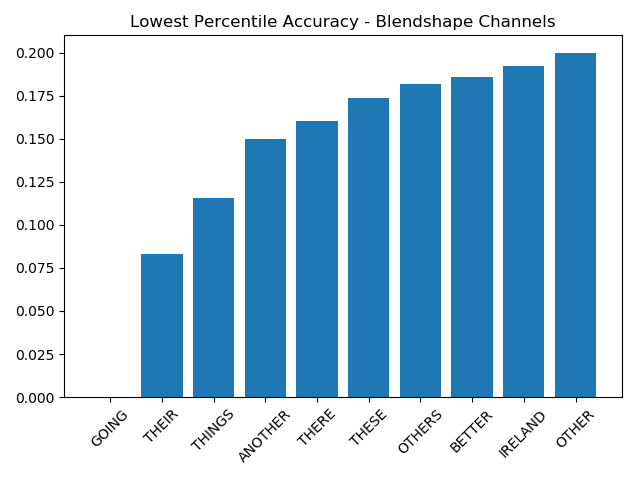
\includegraphics[width=\textwidth]{figures/classification/blendshape_channel_percentile_class_acc.png}
        \caption{Blendshape Channels}\label{fig:channels_percentile_word_acc}
    \end{subfigure}
    \caption{1\textsuperscript{st} Percentile Per Word Test Accuracy}\label{fig:both_models_percentile_word_acc}
\end{figure}

\section{Discussion}
\begin{itemize}
   \item Both models still overfit 
   \item Tuning has increased validation performance but further reduction in overfitting training data causes validation performance to suffer.
   This may be an indication that the data is too similar, this is likely the result of the data source not being as varied as claimed.
   \item Neither model can be said to be better as results are within a small margin of each other. 
   \item Both models got the same wrong wrong >> Could look at this word further.
   \item Both models achieved about 8\% accuracy on all but a single label, 16 times higher than random.
   \item Further work would incorporate context which could improve results
   \item Predict at char level
\end{itemize}
Both weight decay parameters and dropout were applied to both models, however reductions in the deviation between training and validation losses resulted in an overall worse performance on the validation data.
This questions the variation in the dataset?
As mentioned in section \ref{sec:classification_model_arch}, early stopping was applied to both models to halt training once the validation loss has stopped decreasing after ten epochs.